\documentclass[11pt]{article}

\usepackage[margin=1in]{geometry}
\usepackage{amsmath,amssymb}
\usepackage{booktabs}
\usepackage{graphicx}
\usepackage{float}
\usepackage{hyperref}
\graphicspath{{vis_resource/}}

\title{Multicollinearity in 0-Order HAL Basis and Conservative Adjustment}
\author{}
\date{}

\begin{document}
\maketitle

\section{The Problem: Multicollinearity and Flat CVLL}

When using 0-order HAL basis functions (indicator functions / 0-order splines), we encounter multicollinearity when two knots are selected very close to each other. In our experiments (e.g., seed \texttt{11496211}), we observed knot gaps smaller than $10^{-3}$.

\subsection{Mechanism: Multicollinearity and Budget Waste}
When two knots are extremely close (e.g., gap $< 10^{-3}$), the 0-order basis functions become highly correlated. If no validation points fall within this tiny gap, the model can assign large, opposing coefficients (e.g., $+4000$ and $-4000$) to these bases. This configuration cancels out on the observed data, resulting in nearly the same validation likelihood as a model with small coefficients.

However, these large coefficients consume a massive amount of the $L_1$ norm constraint budget. This creates a flat region in the CVLL curve: once the constraint is high enough to fit the signal, further increases are effectively wasted on invisible, cancelling spikes without meaningful improvement in validation likelihood.

\paragraph{Verification (Seed 11496211).}
In this seed, the linear-adjustment initialization selects two extremely close knot pairs:
\[
(0.4910696,\,0.4917118), \qquad (0.5301756,\,0.5303721),
\]
with minimum gap $1.96\times 10^{-4}$. On this dataset, \emph{there are zero observed times} $T$ falling strictly inside either interval, and the same holds fold-by-fold under the Stage-1 CV splitter (5-fold KFold with shuffle and seed).
This makes it possible for the optimization to place large cancelling coefficients on these nearly redundant features without being penalized by the validation log-likelihood.

\subsection{Optuna as a Revealer}
This behavior is not a fault of Optuna itself; Optuna is revealing a pathology in the objective landscape. Because we define a wide search space for the norm constraint (e.g., $[10^{-3}, 10^5]$) to accommodate multiple basis orders, and because the CVLL curve for $k=0$ is flat after the turning point, many large values appear similarly good. As a result, Optuna can select values that are orders of magnitude larger than necessary (e.g., $80{,}000$ instead of $\approx 10$).

\subsection{Verification: Contrast with Higher-Order Bases ($k=1,2$)}
This issue is most severe for the 0-order basis. Higher-order splines ($k=1,2$) are less correlated between adjacent features, so their CVLL curves are better behaved: they rise, peak, then gently decline as overfitting begins.

We verified this by running the same experiment (seed \texttt{11496211}) with basis orders $k=0,1,2$ and plotting CVLL versus the norm constraint.

\begin{figure}[H]
    \centering
    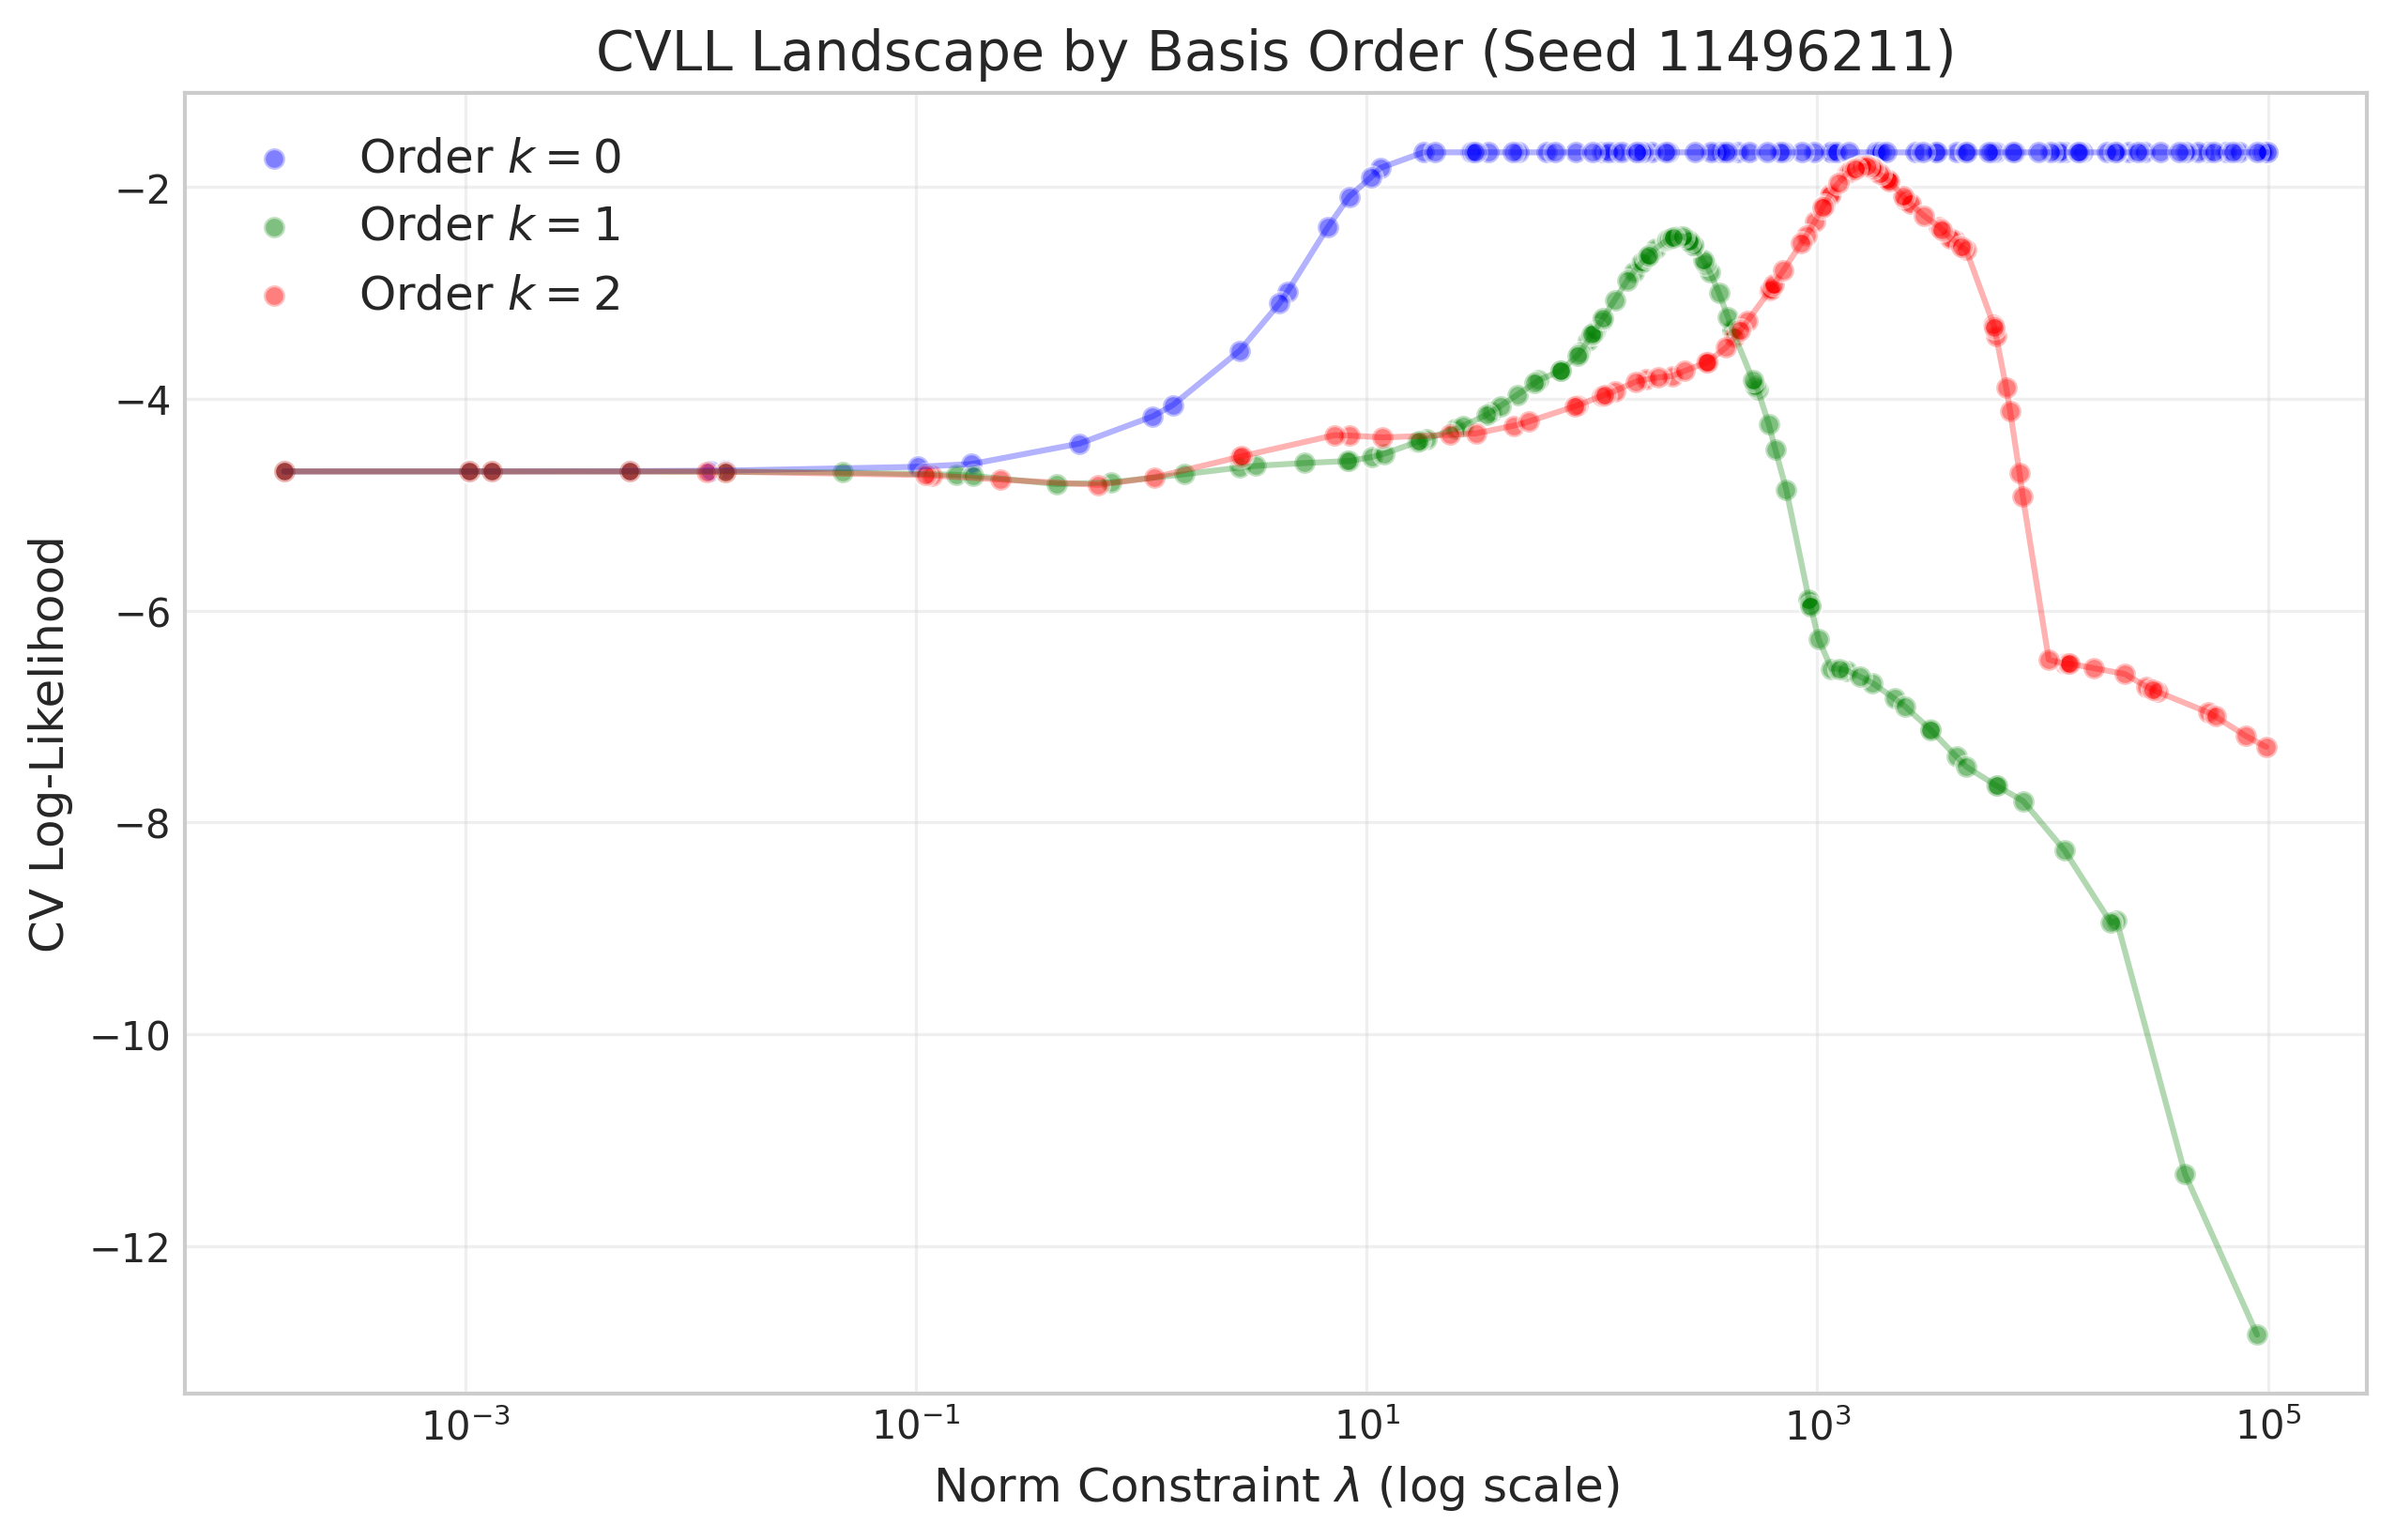
\includegraphics[width=0.82\textwidth]{vis_resource/cvll_by_basis_order.png}
    \caption{CVLL landscape by basis order. The $k=0$ curve exhibits a long plateau, while $k=1,2$ show clearer peak-and-decline behavior.}
    \label{fig:cvll_by_order}
\end{figure}

Figure~\ref{fig:cvll_by_order} shows:
\begin{itemize}
    \item \textbf{Order $k=0$}: the curve rises and then enters a broad plateau (approximately from $\lambda \approx 30$ to $10^5$), so there is no sharp unique optimum.
    \item \textbf{Orders $k=1,2$}: the curves have clearer peaks followed by decline, making the optimal constraint easier to identify.
\end{itemize}

Consistent with the variation interpretation of HAL norms, the scale of the optimal norm constraint increases with basis order:
\begin{itemize}
    \item for $k=1$, peak around $\lambda \approx 240$;
    \item for $k=2$, peak around $\lambda \approx 1600$.
\end{itemize}

\section{Impact on EM Algorithm}
This bad selection can be catastrophic for the subsequent EM step:
\begin{enumerate}
    \item \textbf{Initialization:} with a huge norm (e.g., $\sim 12{,}000$), the initial estimator can place excessive mass on tiny intervals (spikes).
    \item \textbf{EM iterations:} EM starting from this spiky estimate tends to preserve or amplify this allocation, while fitting the rest of the domain nearly constant.
    \item \textbf{Result:} final density quality is severely degraded, sometimes worse than a simple baseline.
\end{enumerate}

\section{The Fix: Conservative Adjustment}
To mitigate this, we use a conservative adjustment strategy: identify the smallest norm constraint on the high-CVLL region near the maximum.

\paragraph{Goal.}
Find the smallest $\lambda$ such that
\[
\mathrm{CVLL}(\lambda) \ge \max_{\lambda'} \mathrm{CVLL}(\lambda') - \mathrm{margin},
\]
where the margin is typically set as a fraction of the CVLL standard deviation (e.g., $5\%$ of SD).

\subsection{Linear Search (Naive)}
The initial approach moved from the Optuna-selected value by a fixed relative decrement (e.g., $2\%$ per step, up to 50 steps).  
If the start is very large (e.g., $12{,}484$), each step is still huge ($\sim 250$), so the search can stop at a still-too-large value ($\sim 250$) and miss the parsimonious region ($\sim 11$).

\subsection{Bisection Search (Robust)}
Replacing linear movement with bisection gives logarithmic refinement and robust behavior across scales. It can efficiently shrink from very large starts to the smallest acceptable $\lambda$.

\section{Empirical Results (Seed 11496211)}

\subsection{Visual Comparison}
Figure~\ref{fig:linear_vs_bisection} compares the resulting density estimates. The linear adjustment gives a spiky poor fit, while bisection gives a smoother estimate close to truth.

\begin{figure}[H]
    \centering
    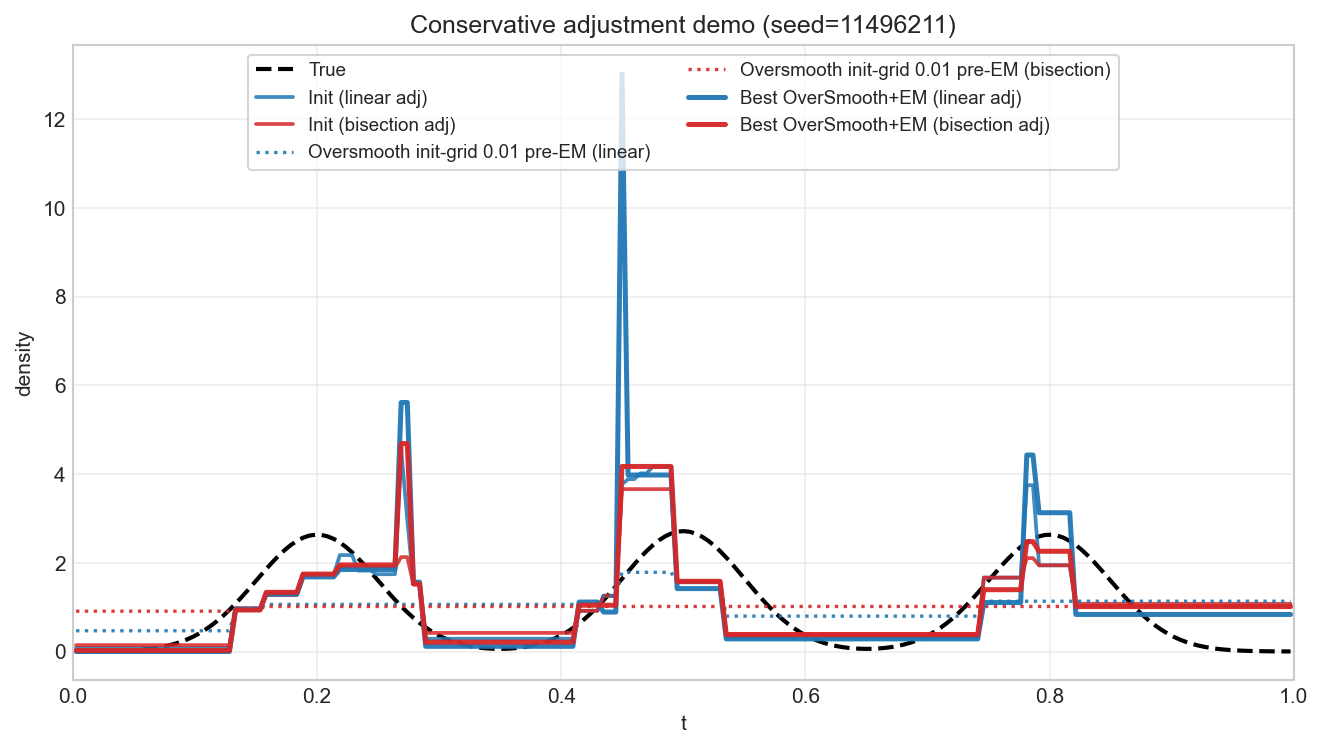
\includegraphics[width=0.82\textwidth]{vis_resource/seed_11496211_linear_vs_bisection.png}
    \caption{Density estimates under linear vs.\ bisection conservative adjustment.}
    \label{fig:linear_vs_bisection}
\end{figure}

\subsection{Metric Comparison}
\begin{table}[H]
    \centering
    \begin{tabular}{lccc}
        \toprule
        Metric & Optuna (No Adj.) & Linear Adj. (Naive) & Bisection Adj. (Robust) \\
        \midrule
        Stage-1 selected norm constraint $\lambda$ & $12484.06$ & $249.68$ & $11.06$ \\
        Stage-1 number of selected knots & $29$ & $29$ & $16$ \\
        Stage-1 max coefficient magnitude $\max|\beta|$ & $2088.71$ & $40.73$ & $1.91$ \\
        Stage-1 $\ell_1$ norm $\|\beta\|_1$ & $12485.32$ & $249.68$ & $11.06$ \\
        Stage-2 best EM KL divergence & $1.03$ & $1.03$ & $0.31$ \\
        Visual quality (Stage-2 best EM) & Spiky, poor fit & Spiky, poor fit & Smooth, close to truth \\
        \bottomrule
    \end{tabular}
    \caption{Three-way comparison: no conservative adjustment (Optuna-selected $\lambda$), naive linear adjustment, and bisection adjustment. Stage-1 rows summarize the initialization estimator; Stage-2 rows summarize the best OverSmooth+EM result.}
    \label{tab:metrics}
\end{table}

In this seed, the Optuna-selected $\lambda$ (no adjustment) yields an initialization with extremely large coefficients (order $10^3$) and a huge $\ell_1$ norm, despite having essentially the same CV objective value as much smaller $\lambda$ values on the plateau. The naive linear adjustment reduces $\lambda$ substantially but can still land on a point that admits tight-knot spikes; the bisection adjustment finds a much smaller $\lambda$ and avoids this pathology.

\subsection{Evidence of Multicollinearity}
In the linear-adjustment run, the solver selected 29 knots with total norm $\sim 250$. Nearby knot pairs carry large opposite coefficients, suggesting cancellation and budget waste:

\begin{table}[H]
    \centering
    \begin{tabular}{cccc}
        \toprule
        Knot index & Location $t$ & Coefficient $\beta$ & Gap to next \\
        \midrule
        $21$ & $0.491070$ & $+38.08$ & $6.4 \times 10^{-4}$ \\
        $22$ & $0.491712$ & $-39.06$ & \dots \\
        \dots & \dots & \dots & \dots \\
        $23$ & $0.530176$ & $+39.14$ & $2.0 \times 10^{-4}$ \\
        $24$ & $0.530372$ & $-40.73$ & \dots \\
        \bottomrule
    \end{tabular}
    \caption{Example close-knot pairs with large cancelling coefficients in the linear-adjustment solution.}
    \label{tab:coef_pairs}
\end{table}

These coefficients (roughly $\pm 40$) consume a large fraction of the norm budget (e.g., $|38| + |-39| \approx 77$) while changing little on observed validation points.

By contrast, the bisection-adjusted solution uses $\lambda \approx 11$, selects only 16 knots, and has maximum coefficient magnitude about $1.91$, preventing this spurious spike behavior.

\subsection{Additional Mechanism Evidence}
Figure~\ref{fig:knot_gaps} shows the consecutive knot gaps for the Stage-1 selected knots: the linear-adjustment initialization contains two gaps below $10^{-3}$ (consistent with the close pairs above), while the bisection-adjustment initialization has none.

\begin{figure}[H]
    \centering
    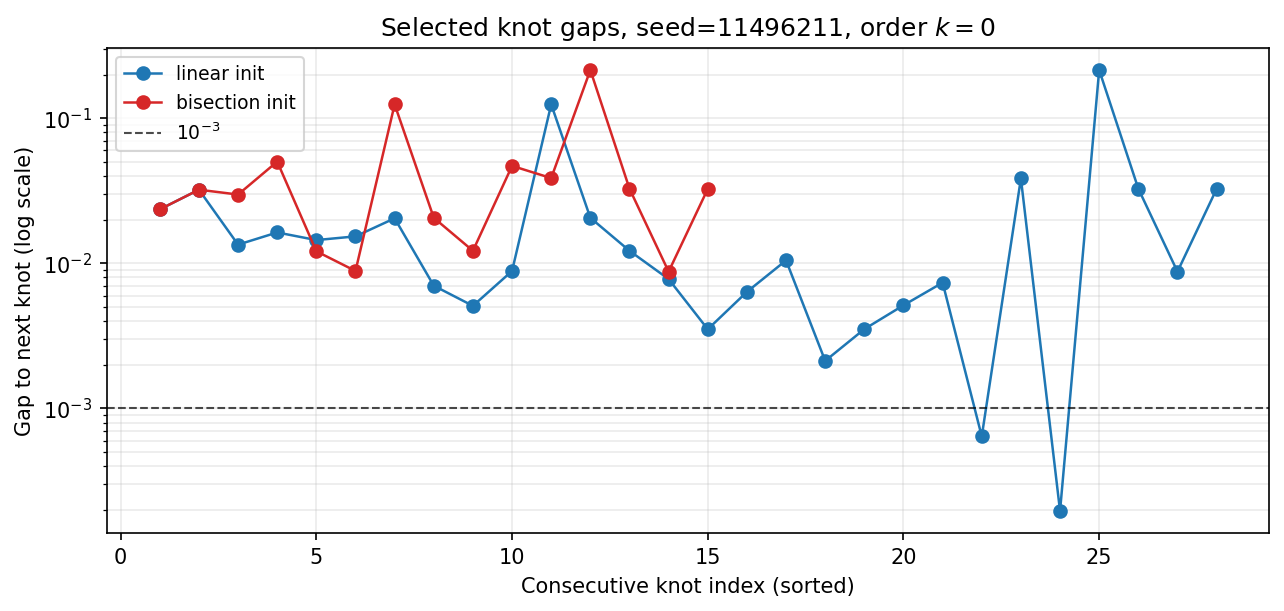
\includegraphics[width=0.82\textwidth]{knot_gaps_linear_vs_bisection.png}
    \caption{Consecutive knot gaps (sorted) in the selected Stage-1 knot sets. Linear adjustment exhibits two gaps $<10^{-3}$; bisection does not.}
    \label{fig:knot_gaps}
\end{figure}

Figure~\ref{fig:coef_abs_hist} shows the coefficient magnitude distribution. In the linear-adjustment initialization, the maximum coefficient magnitude is about $40.7$ and roughly $94.5\%$ of the total $\ell_1$ mass is carried by coefficients with $|\beta|>10$, indicating severe budget concentration. In the bisection-adjustment initialization, the maximum coefficient magnitude is about $1.91$ and the fraction above $10$ is $0$.

\begin{figure}[H]
    \centering
    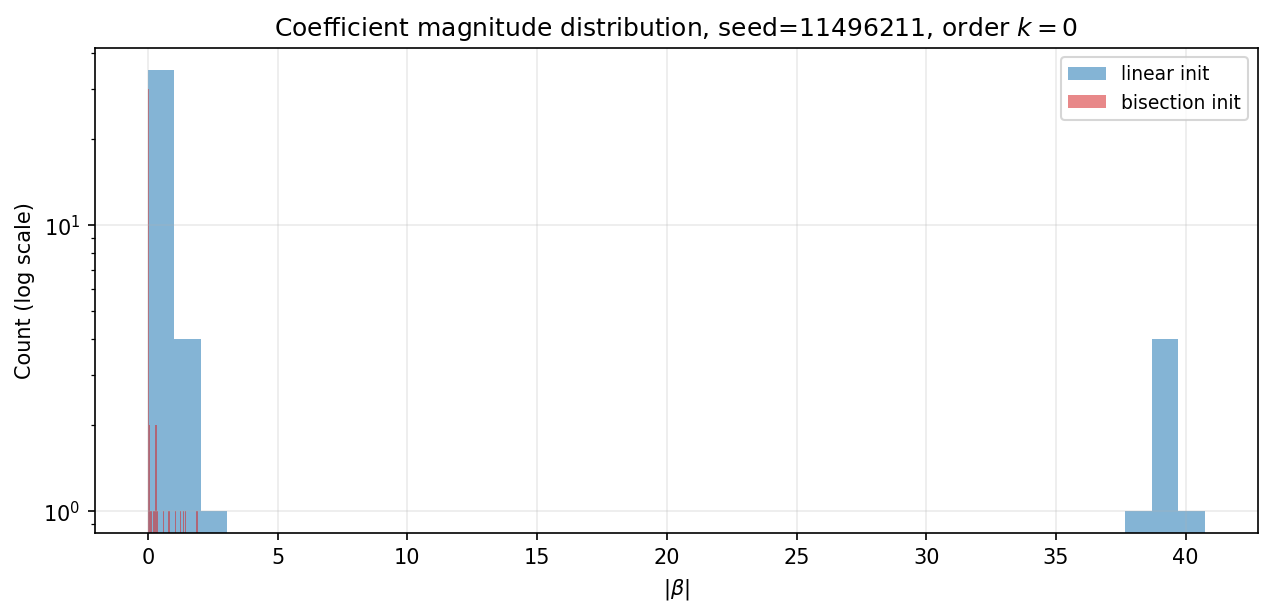
\includegraphics[width=0.82\textwidth]{coef_abs_hist_linear_vs_bisection.png}
    \caption{Histogram of $|\beta|$ for the Stage-1 coefficient vector (log-count scale). Linear adjustment produces large-magnitude coefficients; bisection adjustment does not.}
    \label{fig:coef_abs_hist}
\end{figure}

Finally, Figure~\ref{fig:adj_traces} visualizes the conservative-adjustment trajectories in $(\lambda,\mathrm{CVLL})$ space. The linear search decreases $\lambda$ in coarse multiplicative steps from a very large Optuna proposal (here $\approx 12{,}484$) and can stop at a still-too-large value; bisection efficiently locates a much smaller acceptable $\lambda$ near the turning point.

\begin{figure}[H]
    \centering
    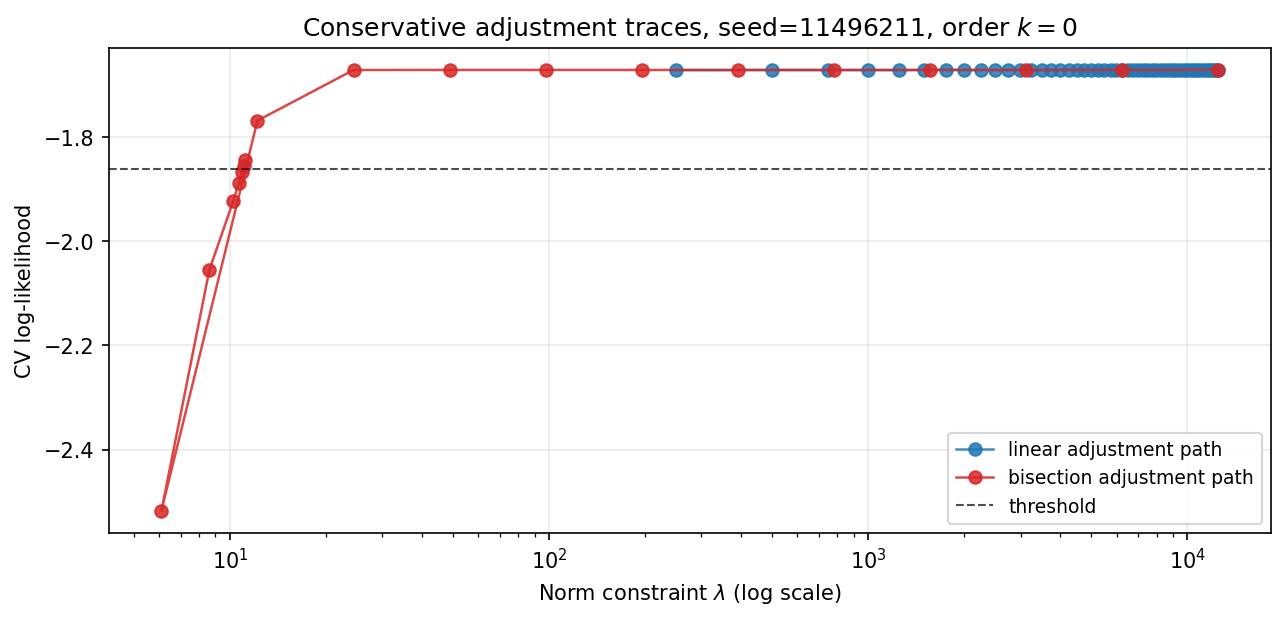
\includegraphics[width=0.82\textwidth]{conservative_adjustment_traces.png}
    \caption{Conservative adjustment traces on the CVLL landscape (seed 11496211).}
    \label{fig:adj_traces}
\end{figure}

\end{document}

